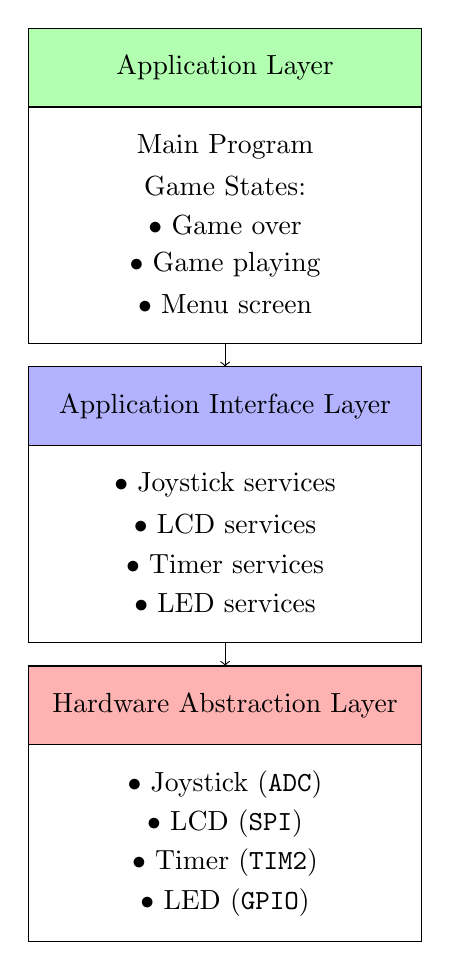
\begin{tikzpicture}
  %first box
  \draw[fill=green!30] (0,0) rectangle (5,-1);
  \draw (0,-1) rectangle (5,-4);
  \draw[->] (2.5,-4) -- (2.5,-4.3);
  %second box
  \draw[fill=blue!30] (0,-4.3) rectangle (5,-5.3);
  \draw (0,-5.3) rectangle (5,-7.8);
  \draw[->] (2.5,-7.8) -- (2.5,-8.1); 
  %third box
  \draw[fill=red!30] (0,-8.1) rectangle (5,-9.1);
  \draw (0,-9.1) rectangle (5,-11.6);


  %titles
  \node at (2.5,-0.5) {Application Layer};
  \node at (2.5,-4.8) {Application Interface Layer};
  \node at (2.5,-8.6) {Hardware Abstraction Layer}; 

  %text in application layer
  \node at (2.5,-1.5) {Main Program};
  \node at (2.5,-2) {Game States:};
  \node at (2.5,-2.5) {$\bullet$ Game over};
  \node at (2.5,-3) {$\bullet$ Game playing};
  \node at (2.5,-3.5) {$\bullet$ Menu screen};
  %text in application interface layer
  \node at (2.5,-5.8) {$\bullet$ Joystick services};
  \node at (2.5,-6.3) {$\bullet$ LCD services};
  \node at (2.5,-6.8) {$\bullet$ Timer services};
  \node at (2.5,-7.3) {$\bullet$ LED services};
  %text in hardware abstraction layer
  \node at (2.5,-9.6) {$\bullet$ Joystick (\texttt{ADC})}; 
  \node at (2.5,-10.1) {$\bullet$ LCD (\texttt{SPI})};
  \node at (2.5,-10.6) {$\bullet$ Timer (\texttt{TIM2})};
  \node at (2.5,-11.1) {$\bullet$ LED (\texttt{GPIO})};  



\end{tikzpicture}